\documentclass[../main.tex]{subfiles}
\begin{document}

The previous chapter ended with the claim that many causal estimators can be constructed to target the same causal estimands and that these estimators may display varied performance under different \textit{distributional settings. }The primary goal of this chapter is to formalize the notion of a \textit{distributional setting }and motivate why the \textit{distributional setting}, as defined, affects estimator performance. In so doing, I will introduce the notion of a causal inference problem space which is the space of all performance-relevant distributional settings.\par

\vspace{\baselineskip}
I will proceed in three steps. First, I will provide a brief overview of the landscape of causal inference estimators. While this overview will include instructive examples of different approaches, it is not meant as a complete (or even partial) review of different methods. Rather, the analysis will provide initial insight into the importance of the properties of the underlying data distribution for the performance of different estimators. The discussion of distributional properties will remain informal at this stage. Second, I will formalize the notion of a distributional setting by expressing causal problems in terms of a joint distribution over observed data. In this context, a distributional setting can then be defined as a joint distribution over the observed data with some set of properties that affect estimator performance. Finally, I will establish the axes of an abstract space over distributional settings with each axis representing different possible values of some property of the joint distribution. This space is the Causal Inference Problem Space.\par

\section{The Sensitivity of Causal Estimators to Properties of the Observed Data}

\vspace{\baselineskip}
In the previous chapter, I arrived at an expression for the average causal effect estimands in terms of  \( E \left[ Y  \vert  X, Z \right]  \)  and referenced this as the ‘response surface’. I also asserted that it was possible to find expressions for the same estimands using meaningfully different, but purely statistical/predictive, estimators. An intuitive explanation for this statement is that causal processes are made up of different \textit{causal} \textit{mechanisms} that relate the various variables\footnote{ Mathematically, these mechanisms take the form of functions which take as inputs some subset of the variables for some unit and output the value of some other variable for that unit. These functions represent some real generative process which relates the measured quantities in the real world. In order to represent real stochastic processes the functions may themselves be stochastic and take the form of distributions parameterized by the input variables. }. And, in order to recover the unbiased effect, it is sufficient to accurately model only one of these mechanisms. Hill (2011) echos this explanation and refers to two mechanisms: the \textit{treatment assignment} \textit{mechanism} - which relates the covariates  \( X \) to the treatment status  \( Z \)  - and the \textit{response} \textit{mechanism} - which relates the covariates  \( X \)  and the treatment status  \( Z \)  to the observed outcome  \( Y \) . The authors point out that an accurate model of either mechanism is sufficient to recover average treatment effects. \cite{Kunzel2019MetalearnersLearning} further divide the \textit{response} mechanism into an \textit{outcome mechanism} which relates the covariates  \( X \) to the outcome without treatment  \( Y_{0} \) and the \textit{treatment effect mechanism} which relates  \( X \) and  \( Z \) to  \(  \tau \) which, in this framing, is the change in outcome (from  \( Y_{0} \) to  \( Y_{1} \) ) as a result of treatment \footnote{ The covariates appear in the treatment effect mechanism because the treatment effect may be non-homogeneous/non-constant in which case it will depend on the covariate values of the exposed unit. }.\  Hypothetically, accurate specification of any of the now three mechanisms is sufficient to recover causal effects. But, given that it is impossible to directly model the treatment effect mechanism without a model of one of the other two mechanisms, it is only useful in so far as it clarifies a potential source of heterogeneity in the combined (outcome and treatment effect) response mechanism as defined by \cite{Hill2011BayesianInference}. With this idea of causal mechanisms in mind, different causal estimators can be understood as arising from the targeting of either, or both, the treatment assignment and response mechanisms. The targeted mechanism also explains the sensitivity of different estimators to different properties of the observed data distribution. With this established, I proceed to the brief overview of different estimators in order to make the points above more tangible.\par


\vspace{\baselineskip}
Looking first at methods which target the treatment assignment mechanism: Matching (\cite{Rosenbaum1983TheEffects}; \cite{Abadie2006LargeEffects}) aims to mitigate selection bias by creating treatment and control groups with the same distribution of covariates, reversing the effect of the treatment assignment mechanism. This is done by pairing units with similar covariate values but different treatment exposure to create two groups with similar overall distributions\footnote{ The reality of the pairing is slightly more nuanced. The standard case is that observed units from a treated group are matched with control units from a ‘donor pool’. This produces an estimate of the average effect for the treated. } \footnote{ Defining a metric in covariate space is a complex task, so there is no single definition of ‘similar’ units. A naive approach is simply to measure the Euclidian distance between covariate vectors in real-number space. Ultimately, a successful metric can be anything which, when applied to large donor pools of observations, results in matches that produce equal covariate distributions across the groups. } \footnote{\cite{Imai2008MisunderstandingsInference} show that if the distribution in the two groups is indeed the same (balanced), then a simple average over the observed outcome is an unbiased estimator of the average treatment effect. }. This process is non-parametric relative to the treatment assignment mechanism because it targets the result of the mechanism without attempting to directly model it\footnote{ Matching methods may indeed have parameters which determine their operation but the correctness of these parameters is independent of the functional form of the treatment assignment mechanism.  }. This means it is not sensitive to the exact functional form of the mechanism. However, it is still sensitive to other aspects of the observed data. \cite{Broomberg2017DeepInference} describes the potential sensitivity as follows. First, as the number of covariates grows, the probability of finding similar units, for any fixed notion of similarity, shrinks exponentially, thus requiring exponentially larger observed donor groups to achieve balance. This holds even in the absence of strong selection pressure producing different covariate distributions between the groups. Second, if there is strong selection pressure, then it is likely that the distribution of covariates will be meaningfully different between the groups. The larger the imbalance, the less likely it will be to find equivalent units in the opposite group and the larger the set of observed units that will be required to find matches. So, in short, matching is sensitive to the number of observed units, the number of covariates, and the functional form of the treatment assignment mechanism (in so far as it affects balance).\par


\vspace{\baselineskip}
Propensity score based methods address some of the weaknesses above by explicitly modeling the treatment assignment mechanism and estimating a probability (propensity) of treatment for each observation. \cite{Austin2011AnStudies} summarizes the various ways in which the propensity score can be used to remove bias. The four classes of methods reviewed by the authors are matching/stratification on the propensity score, inverse probability of treatment weighting, and propensity-based covariate adjustment. These methods share at least two failure modes related to the observed data: one, \cite{Hill2011BayesianInference} points out that the common methods used for estimation of the treatment mechanism are parametric and therefore sensitive to the functional form of the underlying mechanism and the number of covariates. If this form is misspecified, or there are too many covariates, then the resultant propensity scores will not properly mitigate bias. Two, \cite{Knaus2018MachineEvidence} points out that small propensity scores - which inevitably arise when there is an imbalance in covariate distribution across groups - can produce high variance (or even degenerate) estimates in weighting-based methods. So, again, there is sensitivity to the number of covariates, the functional form of the treatment assignment mechanism, and the covariate balance.\par


\vspace{\baselineskip}
Turning to methods which estimate the response surface, a similar pattern of sensitivity is evident. The simplest methods in this class are referred to as conditional mean estimations by \cite{Knaus2018MachineEvidence} or as T-learners by \cite{Kunzel2019MetalearnersLearning}. These methods estimate the conditional mean  \( E \left[ Y \vert  X, Z=z \right]  \)  separately for both the treatment and control groups (a method which was motivated in Chapter \ref{chap:framework}). Much like with direct modeling of the treatment assignment, this approach is sensitive to specification of the function form used for the estimation. This means there is sensitivity to the underlying functional form (and complexity) of the response mechanism. This sensitivity has inspired a huge number of flexible semi/nonparametric estimation schemes. See, for example, Causal Forests by \cite{Athey2018ApproximateDimensions}, BART \cite{Hill2011BayesianInference}, and X-learner \cite{Kunzel2019MetalearnersLearning}. But even these flexible estimation methods are sensitive to aspects of the data distribution. In the case of outcome function fitting, imbalance means that, in both groups, there are certain regions of the covariate support with fewer observations. This makes it hard to accurately fit functions in these regions. This is less problematic in parametric methods with fewer degrees of freedom but seriously affects non-parametric methods which rely on the data for accurate local estimation. Further, response mechanism-based approaches only work if they correctly capture the response dependency on all confounders and the treatment assignment (the treatment effect). This means that, much like in any function fitting task, there is sensitivity to the explainability of the response with respect to the data (the signal-to-noise ratio) and the number of, and redundancy between, predictive variables (the covariates). Incorrect inference of the response mechanism is possible in cases where there is a low signal-to-noise ratio and/or the presence of many covariates with similar but non-identical correlations with the prediction target\par


\vspace{\baselineskip}
The final class of methods explicitly, or implicitly, combines the modeling of both the treatment and response surface, usually through weighted estimation targets. Examples which include explicit models of the two mechanisms are \cite{Rubin2000CombiningCovariates} and \cite{Robins1995SemiparametricData}. \cite{Scharfstein1999AdjustingRejoinder} show that if semiparametric estimation is used for modeling both the treatment assignment and response mechanisms, then the resultant estimators are valid if either the treatment assignment \textit{or }the response mechanism are correctly modeled, leading to the name $``$Double Robust$"$  estimators for this class of methods. Note that while this double robustness is appealing, the models of the two mechanisms are still sensitive to the same aspects of the data as outlined above. The combination simply improves the probability of valid results by hedging the accuracy of the one model with the other. More modern methods may implicitly combine models of both mechanisms rather than explicitly combining them. For example, \cite{Johansson2016LearningInference} jointly optimize a neural network based estimator to produce balanced covariate representations and accurate outcome predictions using this representation. While demonstrating exact sensitivity is hard for complex estimators such as this, it is reasonable to assume that the same sensitivities outlined above will have some impact on accuracy. This is based on the idea that these sensitivities represent fundamental differences in the amount of information available to estimators and the complexity of extracting this information. No estimator, regardless of flexibility or complexity, is immune to the impact of decreasing predictive information.\par


\vspace{\baselineskip}
The synthesis above is, by no means, a complete picture of all the causal estimators present in the literature. Rather, it serves to make a simple point: All estimators - regardless of the mechanism(s) they model and the parametric/non-parametric inference method used to perform the modeling - are sensitive to aspects of the observed data. From the examples above, it appears that the list below is a minimal subset of the performance-relevant aspects of the observed data:\par


\vspace{\baselineskip}
\begin{itemize}
	\item The number of observations\par

	\item The functional forms of the treatment and response mechanism\par

	\item The balance of the covariate distribution across groups\par

	\item The number of covariates\par

	\item The predictive power of the covariates for the treatment assignment/outcome (signal-to-noise ratio and overlap/correlation between predictors)
\end{itemize}\par


\vspace{\baselineskip}
The \textit{distributional setting} of a particular causal inference problem collectively refers to the value of all of these performance-relevant aspects of the observed data. The goal of the next section is to formalize the notion of a distribution setting as a set of properties of the joint distribution over the observed data.

\section{Distributional Settings as Joint Distributions over Observed Data}

\vspace{\baselineskip}
The section above observed that different estimators target different underlying, component mechanisms and that this targeting produces sensitivity to different aspects of the observed data. This section formalizes this idea by showing that the two component mechanisms outlined above can be thought of as acting together to produce a joint distribution over the observed data, with the properties of this distribution affecting estimator performance. In this framing, a \textit{distributional setting }is a joint distribution over the observed data with specific marginal/collective properties that are relevant to performance. Many joint distributions may have the same property values and therefore represent roughly the same distributional setting.\par


\vspace{\baselineskip}
The first step in establishing this framing is to express the component mechanisms discussed above as probability distributions over the variables involved. This is the paradigm used in Pearl’s Structural Causal Models (SCM) \cite{Pearl2009CausalOverview} which builds on the more general idea of representing generative processes as factorized probability distributions that relate causally-connected variables. Readers unfamiliar with these concepts should see \cite{Bishop2006PatternLearning} Chapter 8 for an introduction to graphical models and their interpretation as representing causal, generative processes. In this paradigm, each of the mechanisms above is represented as a conditional distribution:\par


\vspace{\baselineskip}
\begin{itemize}
	\item \textbf{The Treatment Assignment Mechanism:  \( P \left( Z  \vert  X \right)  \) }\par


\vspace{\baselineskip}
	\item \textbf{The Response Mechanism:} in a classic SCM, this would be \( P \left( Y  \vert  Z, X \right)  \) . For consistency with the Potential Outcomes Framework, I further factor  \( P \left( Y  \vert  Z, X \right)  \)  as  \( P \left( Y  \vert  Z, X \right)  = P \left( Y_{1}  \vert  \text{Z , Y}_{0},~ \tau \right) P \left( Y_{0} \vert Z, X \right) P \left(  \tau \vert Z, X \right)  = P \left( Y_{1}  \vert  Y_{0}, \tau \right) P \left( Y_{0} \vert X \right) P \left(  \tau \vert X \right) .  \) This isolates the two sub-mechanisms identified by \cite{Kunzel2019MetalearnersLearning} - the \textit{outcome mechanism }and the \textit{treatment effect }mechanism.\par
\end{itemize}\par

\vspace{\baselineskip}
I add to these mechanisms the idea of an \textit{observation mechanism }which produces the sample of units - both treated and untreated - that are available for study. The \textit{observation mechanism} is not directly useful in revealing the causal effects for the units within the sample but it is important for generalizing the results beyond this group. That is, one can only generalize an inferred effect to a wider population if one assumes the observation mechanism is producing representative samples of the wider population. Further, even if it is not used directly in the causal estimators, this mechanism is an important part of the generative process which produces the observed data and can thus affect estimator performance. For simplicity, I will ignore potential conditioning on a wider population and sampling process and simply refer to a generative distribution over observed units  \( X \) .\par

\begin{itemize}
\vspace{\baselineskip}
	\item \textbf{The Observation Mechanism:  \( P \left( X \right)  \)  }
\end{itemize}\par


\vspace{\baselineskip}
These three conditional distributions - representing the component causal mechanisms - combine to produce a joint distribution over the observed variables:\par


\vspace{\baselineskip}
\begin{adjustwidth}{0.5in}{0.0in}
 \( P \left( X, Y, Z \right)  = P \left( Y \vert X, Z \right) P \left( Z  \vert  X \right) P \left( X \right)  \) \par

\end{adjustwidth}

\begin{adjustwidth}{0.5in}{0.0in}
 \( P \left( X, Y, Z \right)  = P \left( Y_{1}  \vert  \text{Z , Y}_{0},~ \tau \right) P \left( Y_{0} \vert Z, X \right) P \left(  \tau \vert Z, X \right) P \left( Z  \vert  X \right) P \left( X \right)  \) given that  \(  Y=Z \times Y_{1}+ \left( 1-Z \right)  \times Y_{0} \) \par

\end{adjustwidth}


\vspace{\baselineskip}
It is trivially true than any observed dataset can be described by some joint distribution  \( P \left( X, Y, Z \right)  \)  over the variables  \( \text{X, Y} \) and  \( Z \) . Above, I have built this joint distribution from the ‘bottom up’ by defining different component sub-mechanisms of the general causal mechanism, expressing these mechanisms as conditional distributions, and combining them into the joint distribution. An equivalent process for this analysis would be to start from the joint distribution and assert, based on conditional independence implied by some generative model, that the joint distribution can be factored in the way above. The simple but representative generative model in Figure \ref{fig:confounder-scm} of the previous chapter (Chapter \ref{chap:framework}) produces the exact factorization above under the conditional independence relations implied by its structure. The equivalent generation model for the potential outcome based framing is given below in Figure \ref{fig:rubin_generative_model}.\par

\vspace{\baselineskip}

\begin{figure}[ht!]
    \centering
    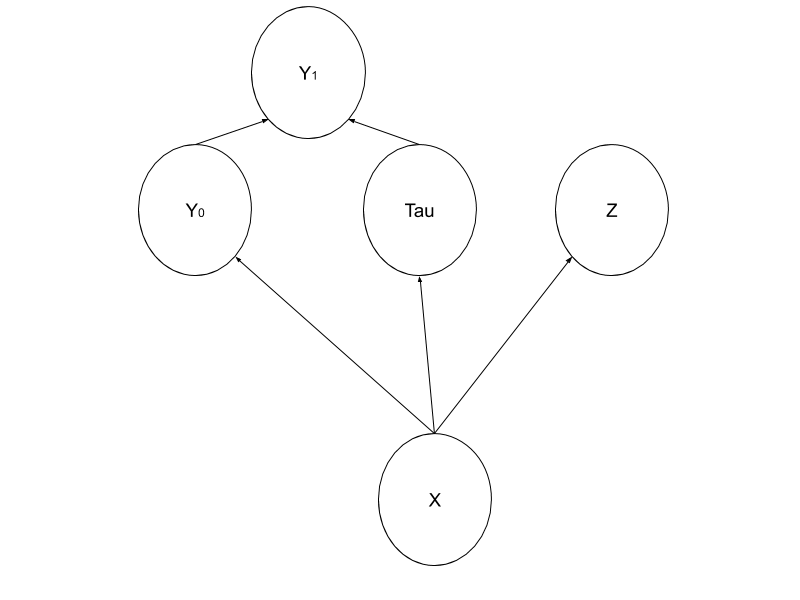
\includegraphics[width=0.7\linewidth]{ch3-rubin-generative-model.png}
    \caption{Graphical (Generative) Model for the variables in Rubin’s potential outcomes framework.}
    \label{fig:rubin_generative_model}
\end{figure}

\vspace{\baselineskip}
With this joint distribution and its factorization in hand, the next conceptual step is to connect the aspects of the observed data discussed above to properties, and factored components, of the distribution. This is relatively straight forward. Some of the aspects of the observed data discussed above relate to properties stemming from a single (factorized) component of the joint distribution. For example, the non-linearity of the outcome mechanism dependents on the functional form of  \( P \left( Y_{0}  \vert  X \right)  \) . Others stem from the combined effect of multiple components. For example, the covariate balance in each group can be described by  \( P \left( X  \vert  Z \right)  \)  which by a simple application of Bayes Theorem is given by the formula below. This formula implies that as the treatment assignment mechanism varies away from simple random assignment  \( P \left( Z \vert X \right)  = 0.5  \forall ~X, \)  the covariate balance in the groups will diverge (as one expects based on intuition).\par


\vspace{\baselineskip}
\begin{adjustwidth}{0.5in}{0.0in}
 \( P \left( X  \vert  Z \right)  \propto P \left( Z  \vert  X \right) P \left( X \right)  \) \par
\end{adjustwidth}

\vspace{\baselineskip}
A complete mapping between the various aspects of the observed data discussed above and properties of the joint distribution is provided later. For now, I simply assert that such a mapping exists based on the motivating examples above. The question then becomes why framing the different aspects of the data discussed above in terms of the joint distribution is useful.\par

\vspace{\baselineskip}
There are three reasons for this. Firstly, it unifies conceptually disparate aspects of the observed data - functional form, covariate balance, predictive power etc - into a single theoretical object. The joint distribution fully determines the aspects of the data which impact performance. Thus, the \textit{distributional setting }can be used to coherently describe a class of joint distributions which reliably result in similar estimator performance characteristics. All joint distributions with similar, quantitatively-defined properties - that is, with the same distributional setting - should exhibit similar performance. Second, this framing provides a clear connection between the process used to generate the observed data, the observed data itself, and the performance of estimators. The introduction briefly mentioned that Monte Carlo methods can sample from flexibly-specified joint distributions. The dependence of estimators on the joint distribution over  \( \text{X, Y} \) , and  \( Z \)  - as established here - is what results in Monte Carlo being a useful evaluation tool. Monte Carlo sampling can be used to generate joint distributions corresponding to different distributional settings in which estimators can be expected to perform quite differently relative to each other and to their performance in other settings. Third, combining these two reasons, a concrete notion of distributional setting allows for the construction of an explorable causal inference problem space. The abstract problem space contains all of the meaningfully different distributional settings (those with different impact on estimator performance) and the use of Monte Carlo generative processes allows for the exploration of this space in order to validate estimators in a (theoretically) exhaustive set of circumstances. Establishing this space is the focus of the next section.\par

\section{The Causal Inference Problem Space}

\vspace{\baselineskip}
The first section in this chapter used examples of estimators to highlight sensitivity to aspects of the observed data. The second section introduced the idea that the performance-relevant aspects of the observed data can be fully described in terms of a \textit{distributional setting} which describes the properties of the joint distribution  \( P \left( X, Y, Z \right)  \). This section brings these ideas together by describing the so-called axes which define the space of distributional settings eluded to at the end of the last section. The axes introduced below represent the properties of the joint distribution which can vary and, in doing so, produce changes in the performance of estimators when applied to the corresponding data. The resultant problem space is intended to be exhaustive, implying that the axes should span all \textit{distinct problem classes - }classes of joint distributions which yield different estimator performance. The claim that the defined space is exhaustive is hard to prove concretely. Indeed, I expect that iteration on the axes may be required to meet the goal of defining an appropriate basis. However, it is worth noting two points which motivate the choice of axes below:\par


\vspace{\baselineskip}
\begin{itemize}
	\item The axes were selected in a principled manner by examining the properties of the joint distribution affected by manipulation of the underlying mechanisms described in the last two sections - the treatment assignment mechanism and the outcome mechanism. This is not a guarantee that all relevant distributional properties have been discovered but it does mean those selected are non-arbitrary and arise from varied causal mechanisms.\par


\vspace{\baselineskip}
	\item The axes selected by this principled process end up spanning the evaluation settings present in the benchmarking literature that is reviewed in Chapter \ref{chap:litreview}. This means that, at a minimum, these axes span the space of settings present in a wide sample of the relevant literature even if the resultant (sub)space is not exhaustive of the full problem space.
\end{itemize}\par


\vspace{\baselineskip}
Finally, it is worth noting that, while I do not present them here, each axis has at least one associated metric which assigns it a specific value for any given joint distribution. If the axes do span the causal inference problem space,  and the metrics successfully measure each axis, then combinations of these metric values should be able to represent every distinct class of causal inference problem.\par

%%%%%%%%%%%%%%%%%%%%%%%%%% AXES %%%%%%%%%%%%%%%%%%%%%%%%%

\vspace{\baselineskip}
Without further ado, I present the proposed axes of the causal inference problem space. For each axis, I explain which distributional component(s) of the overall causal mechanism affect its value. Following each definition (or group of related definitions), I provide simple toy datasets and estimators to demonstrate the impact of the axis on estimator performance. The toy datasets are based on a single covariate  \( X \) and use the simplest possible setting for all axes but the one in focus.\par


\vspace{\baselineskip}
\begin{enumerate}
	\item \textbf{The Nonlinearity (Modeling Complexity) of the (Untreated) Outcome Mechanism} which defines the distribution over the value of  \( Y_{0} \)  (the outcome without treatment) based on a unit’s covariates. This corresponds to the functional form of the distribution  \( P \left( Y_{0}  \vert  X \right)  \). \par


\vspace{\baselineskip}
	\item \textbf{The Nonlinearity (Modeling Complexity) of the Treatment Effect Mechanism} which defines the distribution over the treatment effect for each unit. This corresponds to the form of the distribution  \( P \left(  \tau  \vert  X \right)  \)  and specifically the dependence on the covariates  \( X \) . \par

\uline{Toy Example for the Nonlinearity of the Response Mechanism}\par

\vspace{\baselineskip}

The example below demonstrates the impact of a nonlinear response mechanism - created by nonlinearity in either or both of the untreated outcome or the treatment effect - when using parametric (potentially misspecified) conditional mean regression. This example is inspired by a similar plot found in \cite{Hill2011BayesianInference}. It is evident that the misspecification of the regression model used to model the outcomes in each group produces an estimation error.

\vspace{\baselineskip}

It is worth noting that this toy example glosses over some nuance. First, the error depicted only applies to estimates of the individual treatment effect. Estimates of average effects will be unbiased in this case as a result of the balance of the covariates across the treatment groups. (The average effect estimate in the example below is, indeed, 0). Second, depending on the modeling approach used, nonlinearity in the treatment effect mechanism may not have the same result as nonlinearity in the outcome mechanism. The point of this example is simply to demonstrate that there is sensitivity to the nonlinear of the outcome mechanism.

\vspace{\baselineskip}

\begin{figure}[ht!]
    \centering
    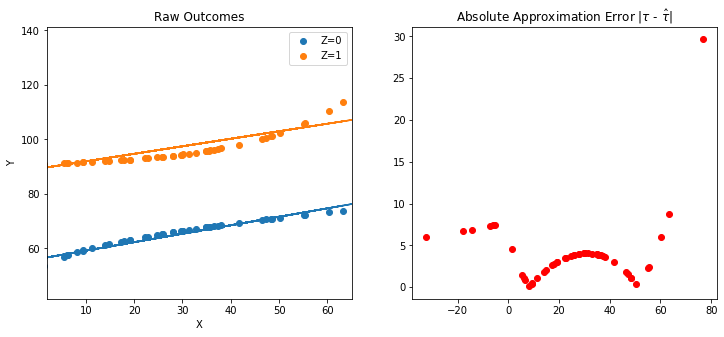
\includegraphics[width=0.85\linewidth]{figures/ch3-nonlinearity.png}
    \caption{Left panel: the covariate and outcome values for the nonlinear response mechanism toy example. The data is divided into treatment groups with a linear outcome model plotted for each group. Right panel: the absolute error in the predicted individual treatment effect for each observation in the dataset. It is clear that a nonlinear outcome mechanism, combined with a misspecified outcome model, produces bias in the effect estimation.}
    \label{fig:toy-1}
\end{figure}
\FloatBarrier

\par

\vspace{\baselineskip}
	\item \textbf{The Magnitude of the Treatment Effect:} the magnitude of treatment effect, measured relative to noise in the outcome mechanism (as defined above). This corresponds to the magnitude of the values produced by \( P \left(  \tau  \vert  X \right)  \) and the magnitude of the noise in  \( P \left( Y_{0}  \vert  X \right)  \)  - IE, the changes in  \( Y_{0} \) not correlated with changes in  \( X. \) \par


\vspace{\baselineskip}

\vspace{\baselineskip}
\uline{Toy Example for Magnitude of Treatment Effect}

\vspace{\baselineskip}
The example below demonstrates the impact of a treatment effect which is small relative to the noise in the outcome mechanism. The base outcome is linear and the treatment effect is constant. This is a classically easy problem but, in this case, the noise makes correctly-specified parametric inference highly inaccurate.\par

\vspace{\baselineskip}

\begin{figure}[ht!]
    \centering
    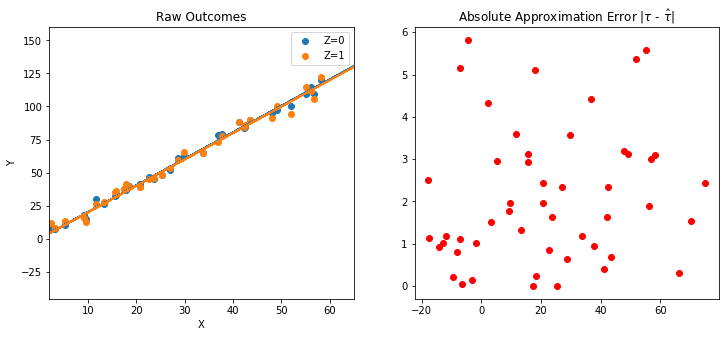
\includegraphics[width=0.85\linewidth]{figures/ch3-noise.png}
    \caption{Left panel: the covariate and outcome values for the magnitude of treatment effect toy example. The data is divided into treatment groups with a linear outcome model plotted for each group. Right panel: the absolute error in the predicted individual treatment effect for each observation in the dataset. It is clear that a low signal-to-noise ratio produced by treatment effect values that are small relative to the outcome noise produces bias in the effect estimation. }
    \label{fig:toy-2}
\end{figure}
\FloatBarrier

\vspace{\baselineskip}
	\item \textbf{The Nonlinearity/Complexity of the Treatment Assignment Mechanism} which defines the distribution over the treatment assignment value based on a unit’s covariates. This corresponds to the form of \( P \left( Z  \vert  X \right)  \) , the treatment assignment mechanism per the definitions above.

\vspace{\baselineskip}
This can have an effect in one of two ways. In methods which directly model the treatment assignment mechanism to reverse selection bias, misspecification (of a more complex function) will induce bias. In methods which don’t model the treatment assignment, a nonlinear assignment will (likely) result in more extreme propensity scores. This will produce regions of the covariate space with imbalance/the absence of overlap.

\vspace{\baselineskip}
The second situation is displayed in the toy example below. A non-linear treatment assignment logit - in this case a simply cubic around the mean value of the covariate X - produces treatment groups with little to no overlap. This results in error despite the correctly specified outcome model.

\vspace{\baselineskip}
\tab \uline{Toy Example for Nonlinearity of Treatment Assignment Mechanism}\par


\vspace{\baselineskip}

\begin{figure}[ht!]
    \centering
    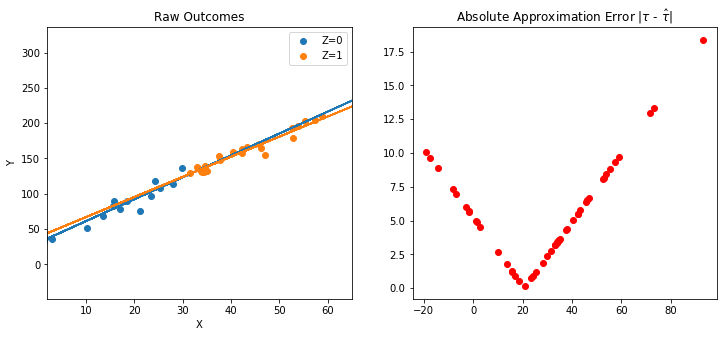
\includegraphics[width=0.85\linewidth]{figures/ch3-treat-nonlinearity.png}
    \label{fig:toy-treat-nonlin}
\end{figure}
\FloatBarrier


\vspace{\baselineskip}
	\item \textbf{The Covariate Balance:} The (dis)similarity of the distributional of covariates in the two treatment groups. As above, this is determined by  \( P \left( Z \vert X \right)  \) and  \( P \left( X \right)  \). \par

\vspace{\baselineskip}
	\item \textbf{Covariate Distribution Overlap} this is conceptually similar to balance but refers to whether the domain of the covariate distribution in each of the treatment groups is the same. Much like balance it is determined by  \( P \left( Z \vert X \right)  \) and  \( P \left( X \right)  \).

\vspace{\baselineskip}

In finite samples, the impact of imbalance and lack of overlap is similar, so a single toy example is given below. However, in the asymptotic limit, appropriate methods can reverse the bias induced by imbalance but will not reverse the bias induced by lack of overlap. This is why overlap was taken as a strong assumption of valid causal inference in Chapter \ref{chap:framework}.

\vspace{\baselineskip}

\uline{Toy Example for the Balance and Overlap Axes}\par

\vspace{\baselineskip}
The example below demonstrates the effect of covariate imbalance induced through strong selection pressure. The example outcome is a simple linear model with a constant treatment effect and moderate noise. Strong selection pressure is simulated by filtering the treated/control observations which fall outside of the indicated overlap region. This produces treatment groups with an unbalanced distribution of the covariate X. This results in conditional regressions that extrapolate beyond the bounds of the outcome information. When combined with moderate noise, this produces large error outside of the region of overlap between the groups.\par

\vspace{\baselineskip}

\begin{figure}[ht!]
    \centering
    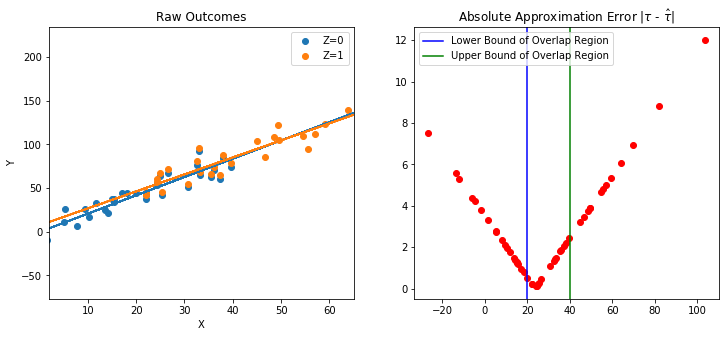
\includegraphics[width=0.85\linewidth]{figures/ch3-balance.png}
    \caption{Left panel: the covariate and outcome values for the balance/overlap toy example. The data is divided into treatment groups with a linear outcome model plotted for each group. Right panel: the absolute error in the predicted individual treatment effect for each observation in the dataset. It is clear that, with a finite sample size, imbalance between the treatment groups’ covariate distributions produces bias in the effect estimation.}
    \label{fig:toy-3}
\end{figure}
\FloatBarrier

\par

\vspace{\baselineskip}

\vspace{\baselineskip}
	\item \textbf{The Percent of Units Treated: }the\ (dis)similarity of the number of units in each group stemming from systematically extreme (low or high) values of the probability for treatment for all observed units. Again, primarily determined by  \( P \left( Z \vert X \right)  \) and  \( P \left( X \right)  \) .\par


\vspace{\baselineskip}
\uline{Toy Example for the Percent of Units Treated}\par

\vspace{\baselineskip}
The example below demonstrates the effect of a small percent of units treated. It was created by giving all units a small probability of treatment - set at $P(T|X) = 0.1$.The result is similar to the case of imbalance, in that there is imperfect overlap that results in extrapolation. But, in this case, this lack of overlap is created simply by a small treated group even though covariate balance holds in the asymptotic limit. IE, if there were many more observations, and the same fixed but small propensity for treatment, the bias would dissapear.

\vspace{\baselineskip}

\begin{figure}[ht!]
    \centering
    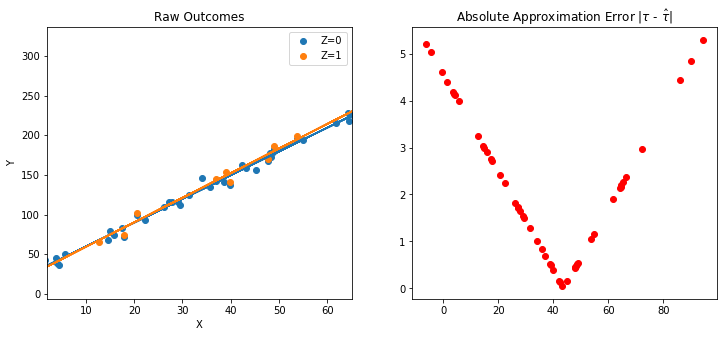
\includegraphics[width=0.85\linewidth]{figures/ch3-percent-treated.png}
    \caption{Left panel: the covariate and outcome values for the small percent of treated units toy example. The data is divided into treatment groups with a linear outcome model plotted for each group. Right panel: the absolute error in the predicted individual treatment effect for each observation in the dataset. It is clear that, with a finite sample size, a small treated group produces bias in the effect estimation.}
    \label{fig:toy-4}
\end{figure}
\FloatBarrier
\par

\vspace{\baselineskip}
	\item \textbf{The Degree of Alignment Between the Treatment Assignment and Outcome Mechanism:} the number of confounding covariates - that appear in both the treatment assignment and outcome mechanisms - relative to the number of non-confounding, but still, predictive covariates - that appear in at least of the two mechanisms. The term alignment, to reflect this degree of confounding, is taken from \cite{Kern2016AssessingPopulations}.

\vspace{\baselineskip}

The impact of this axis is subtle. If there are a small number of confounders relative to the variables that are predictive of either (but not both) of the treatment assignment and outcome, then controlling for confounding becomes a difficult variable selection problem. It is possible that a model may accurately model both the treatment and outcome mechanism without controlling for the confounding effect of a few variables even if the mechanism by which these variables affect treatment assignment/outcome is relatively simple. Conversely, if there is a large number of confounders relative to the predictive covariates then variable selection is easier but modeling the treatment/outcome mechanisms (or reversing bias by other means) is more challenging. This complexity means that this axis does not lend itself to simple demonstration through a toy example. I defer quantitative demonstration for Chapter \ref{XXX}, which presents results from a benchmark that varies the alignment axis of the distributional setting.


\vspace{\baselineskip}
	\item \textbf{Other Axes:} there are two further properties of observed data that are relevant to estimator performance but are not strictly properties of the joint distribution. These properties are ignorability - whether all covariates which make up the treatment and outcome mechanisms are observed - and the number of observed samples - that, as was clear from the above, modulates the effect of many of the other axes. Given their close relation to the joint distribution, and their impact on performance, I treat these two properties as axes of the distributional setting problem space.\par

\end{enumerate}

\section{Conclusion}

This chapter laid the theoretical groundwork necessary for the robust evaluation of causal inference estimators. Different estimators target different components of the causal mechanism and this produces sensitivity to different properties of the joint distribution over the observed data. The Causal Inference Problem Space is a space defined by ten axes along which the properties of the joint distribution vary. Understanding this space is important because different estimators are likely to perform differently on distributions which lie in different parts of it. With this foundation established, the next chapter goes on to review the methods used to evaluate causal inference methods in the literature.

\end{document}